
\documentclass{beamer}

%\usepackage[table]{xcolor}
\mode<presentation> {
  \usetheme{Boadilla}

%  \usetheme{Pittsburgh}
%\usefonttheme[2]{sans}
\renewcommand{\familydefault}{cmss}
%\usepackage{lmodern}
%\usepackage[T1]{fontenc}
%\usepackage{palatino}
%\usepackage{cmbright}
  \setbeamercovered{transparent}
\useinnertheme{rectangles}
}

\setbeamercolor{normal text}{fg=black}
\setbeamercolor{structure}{fg= blue}
\definecolor{trial}{cmyk}{1,0,0, 0}
\definecolor{trial2}{cmyk}{0.00,0,1, 0}
\definecolor{darkgreen}{rgb}{0,.4, 0.1}
\usepackage{array}
\beamertemplatesolidbackgroundcolor{white}  \setbeamercolor{alerted
text}{fg=red}
\usepackage{tcolorbox}
\setbeamertemplate{caption}[numbered]\newcounter{mylastframe}


\usepackage{tikz}
\usetikzlibrary{arrows}
\usepackage{colortbl}

\renewcommand{\familydefault}{cmss}
%\usepackage[all]{xy}

\usepackage{tikz}
\usepackage{lipsum}

 \newenvironment{changemargin}[3]{%
 \begin{list}{}{%
 \setlength{\topsep}{0pt}%
 \setlength{\leftmargin}{#1}%
 \setlength{\rightmargin}{#2}%
 \setlength{\topmargin}{#3}%
 \setlength{\listparindent}{\parindent}%
 \setlength{\itemindent}{\parindent}%
 \setlength{\parsep}{\parskip}%
 }%
\item[]}{\end{list}}
\usetikzlibrary{arrows}

\usecolortheme{lily}

\newtheorem{com}{Comment}
\newtheorem{lem} {Lemma}
\newtheorem{prop}{Proposition}
\newtheorem{condition}{Condition}
\newtheorem{thm}{Theorem}
\newtheorem{defn}{Definition}
\newtheorem{cor}{Corollary}
\newtheorem{obs}{Observation}
 \numberwithin{equation}{section}
 

\setbeamertemplate{navigation symbols}{}


\title[PLSC 43401]{Mathematical Foundations of Political Methodology}

\author{Robert Gulotty}
\institute[Chicago]{University of Chicago}
\vspace{0.3in}




\begin{document}

\begin{frame}
\maketitle
\end{frame}


\begin{frame}
\frametitle{Day 5: Summarizing Random Variables}

\begin{itemize}
\item Covariance
\item Multivariate Distributions
\item Law of Iterated Expectations (LIE)
\item Law of Total Variance
\end{itemize}
\end{frame}




\begin{frame}
\frametitle{Conditional Probability Distribution Function}


\begin{defn}
Suppose $X$ and $Y$ are continuous random variables with joint pdf $f(x,y)$.  Then define the \alert{conditional probability function} $f(x|y)$ as 

\begin{eqnarray}
f(x|y) & = & \frac{f(x, y) }{f_{Y}(y) } \nonumber 
\end{eqnarray}

\end{defn}




\end{frame}

\begin{frame}
\frametitle{Covariance} 

\begin{defn} 
For jointly continuous random variables $X$ and $Y$ define, the covariance of $X$ and $Y$ as,\pause 
\begin{eqnarray}
\invisible<1>{\text{cov}(X,Y) & = & E[(X-E[X])(Y- E[Y])] \nonumber} \pause  \\
\invisible<1-2>{& = & E\left[ XY - E[X] Y - E[Y] X + E[X]E[Y] \right] \nonumber} \pause  \\
\invisible<1-3>{& = & E[XY] - 2E[X]E[Y] + E[E[X]E[Y]] \nonumber } \pause \\
\invisible<1-4>{& = & E[XY] - E[X]E[Y] \nonumber } \pause 
\end{eqnarray}
\invisible<1-5>{Define the correlation of $X$ and $Y$ as, } \pause 
\begin{eqnarray}
\invisible<1-6>{\text{cor}(X,Y) & =&  \frac{\text{cov}(X,Y) }{\sqrt{\text{Var}(X) \text{Var}(Y) } } \nonumber } 
\end{eqnarray}
\end{defn} 

\end{frame}


\begin{frame}
\frametitle{Some Observations}

Variance is the covariance of a random variable with itself.\pause 
\begin{eqnarray}
\invisible<1>{cov(X,X) & = & E[X X] - E[X]E[X] \nonumber} \\
\invisible<1>{& = & E[X^2] - E[X]^2 \nonumber }
\end{eqnarray}
\pause 
\invisible<1-2>{Correlation measures the linear relationship between two random variables\\} \pause 
\invisible<1-3>{Suppose $X = Y$} \pause 
\begin{eqnarray}
\invisible<1-4>{cor(X,Y) & = & \frac{cov(X,Y)}{\sqrt{Var(X)Var(Y)} } \nonumber \\} \pause 
\invisible<1-5>{& = & \frac{Var(X)}{Var(X)} \nonumber \\} \pause 
\invisible<1-6>{& = & 1 \nonumber } \pause 
\end{eqnarray}

\invisible<1-7>{Suppose $X = -Y$ } \pause 
\begin{eqnarray}
\invisible<1-8>{cor(X,Y) & = & \frac{cov(X,Y)}{\sqrt{Var(X)Var(Y)} } \nonumber \\} \pause 
\invisible<1-9>{& =  & \frac{- Var(X)}{Var(X)} \nonumber \\} 
\end{eqnarray}

\end{frame}

\begin{frame}{Plot pdf $f(x,y)=x+y$}

x $<$- seq(0, 1, 0.01)\\
y $<$- seq(0, 1, 0.01)\\
z $<$- outer(x, y, function(x, y)\{ x + y \})\\
persp(x, y, z)

\end{frame}


\begin{frame}
\includegraphics[width=4 in]{roof.pdf}

\end{frame}


\begin{frame}
\frametitle{Example: $X + Y$} 
Suppose $X$ and $Y$ have pdf $x + y$ for $x, y \in [0,1]$.  \pause \\
\invisible<1>{Cov$(X,Y)$ } \pause 
\begin{eqnarray}
\invisible<1-2>{E[XY] & = & \int_{0}^{1} \int_{0}^{1} xy (x + y) dx dy \nonumber } \pause \\
\invisible<1-3>{& = & \int_{0}^{1} \int_{0}^{1} (x^2 y + y^2 x) dx dy \nonumber } \pause \\
\invisible<1-4>{& = & \int_{0}^{1} (\frac{y}{3} + \frac{y^2}{2} ) dy \nonumber } \pause \\
\invisible<1-5>{& = & \frac{1}{6} + \frac{1}{6} = \frac{1}{3} \nonumber} \pause  
\end{eqnarray}

\begin{eqnarray}
\only<1-8>{\invisible<1-6>{E[X] & = & \int_{0}^{1} \int_{0}^{1} x (x + y) dxdy \nonumber } \pause \\
\invisible<1-7>{ & = & \frac{7}{12} \nonumber } } 
 \only<9-10>{E[Y] & = & \int_{0}^{1} \int_{0}^{1} y(x + y) dxdy \nonumber \pause \\
 & = & \invisible<1-9>{\frac{7}{12} \nonumber }} 
 \end{eqnarray}
\pause 

\end{frame}




\begin{frame}
\frametitle{Example: $X + Y$ } 

\begin{eqnarray}
\text{Cov}(X,Y) & = &  E[XY] - E[X]E[Y] \nonumber  \pause \\
\invisible<1>{& = & \frac{1}{3}  - \frac{49}{144} = -\frac{1}{144} \nonumber } \pause 
\end{eqnarray}

\begin{eqnarray}
\invisible<1-2>{\text{Cor}(X,Y) & = & \frac{\text{Cov}(X,Y)}{\sqrt{\text{Var}(X) \text{Var}(Y) }} \nonumber } \pause \\
\invisible<1-3>{& = & \frac{- \frac{1}{144}}{\frac{11}{144}} \nonumber} \pause  \\
\invisible<1-4>{& = & \frac{-1}{11} \nonumber}  
\end{eqnarray}


\end{frame}


\begin{frame}
\frametitle{Conditional Expectation}
$$\mathbb{E}(Y|X)=\int y\cdot f_{Y|X} (y|x)dy $$
$\mathbb{E}(Y|X)$ is the \emph{best} way to predict Y given X.

\end{frame}




\begin{frame}
\frametitle{Example of Joint Density}
$$f_{X,Y}(x,y) = x+y,\ \quad for\ x,\ y\ \in [0,1]$$\pause
the marginal densities $f_X(x)$ and $f_Y(y)$ are
$$f_X(x)=x+\frac{1}{2}$$\pause
$$f_Y(y)=\frac{1}{2}+y$$\pause
$$f_{X|Y}(x|y)=\frac{f_{X,Y}(x,y)}{f_Y(y)}=\frac{x+y}{\frac{1}{2}+y}$$
\end{frame}




\begin{frame}
\includegraphics[width=4 in]{roof.pdf}

\end{frame}



\begin{frame}
\frametitle{Example of Conditional Expectation}
$$E(Y|X)=\int_0^1 y f_{Y|X}(y|x)dy$$\pause
$$=\int_0^1 y \big(\frac{x+y}{\frac{1}{2}+x}\big)dy$$\pause
$$=\frac{1}{x+\frac{1}{2}}\int_0^1 y (x+y)dy$$\pause
$$=\frac{1}{x+\frac{1}{2}} \big(\frac{y^2x}{2} +\frac{y^3}{3}\big) |_0^1$$\pause
$$=\frac{2+3x}{3+6x}$$
\end{frame}




\begin{frame}
\frametitle{Best Linear Predictor}
Suppose we want a predictor $E(Y|X)$ that is linear:
$$f(X)=a+bX$$
Where $a$ and $b$ are set to minimize
$$E[(Y-(a+bX))^2]$$

\end{frame}

\begin{frame}
\frametitle{Best Linear Predictor}
$$E[(Y-(a+bX))^2]$$\pause
Take partial derivative with respect to $a$.\pause
$$\partial E[(Y-(a+bX))^2]/\partial a= E[\partial(Y-(a+bX))^2/\partial a]$$\pause
$$= -2E[(Y-(a+bX))]$$\pause
setting equal to 0:\pause
$$0= -2E[(Y)-(a+bX)]$$\pause
$$0= -2E[Y]+2E(a+bX)]$$\pause
$$E[Y]=a+bE(X)$$\pause
$$E[Y]-bE(X)=a$$
\end{frame}

\begin{frame}
\frametitle{Best Linear Predictor}
$$E[(Y-(a+bX))^2]$$\pause
Take partial derivative with respect to $b$.\pause
$$\partial E[(Y-(a+bX))^2]/\partial b= E[\partial(Y-(a+bX))^2/\partial b]$$\pause
$$= 2E[(Y-(a+bX))(-X)]$$\pause
setting equal to 0:\pause
$$0= -2E[(YX)-(a+bX)(X)]$$\pause
$$0= -2E[YX]+2E(a+bX)(X)]$$\pause

\end{frame}
\begin{frame}{Best Linear Predictor (continued)}
$$E[YX]=aE(X)+bE(X^2)]$$\pause
$$E[YX]=[E[Y]-bE(X)]E(X)+bE(X^2)]$$\pause
$$E[YX]=E[Y]E(X)-bE(X)E(X)+bE(X^2)]$$\pause
$$E[YX]-E[Y]E(X)=b[E(X^2)-E[X]^2]$$\pause
$$b=\frac{E[YX]-E[Y]E(X)}{[E(X^2)-E[X]^2]}=\frac{Cov(X,Y)}{Var(X)}$$
\end{frame}



\begin{frame}
\frametitle{Best Linear Predictor}
Example: $X + Y$\\
Suppose $X$ and $Y$ have pdf $x + y$ for $x, y \in [0,1]$.  \pause \\

$$b=\frac{cov(X,Y)}{Var(X)} = -1/11$$
$$a=E(Y)-bE(X)= 84/132$$
\end{frame}


\begin{frame}
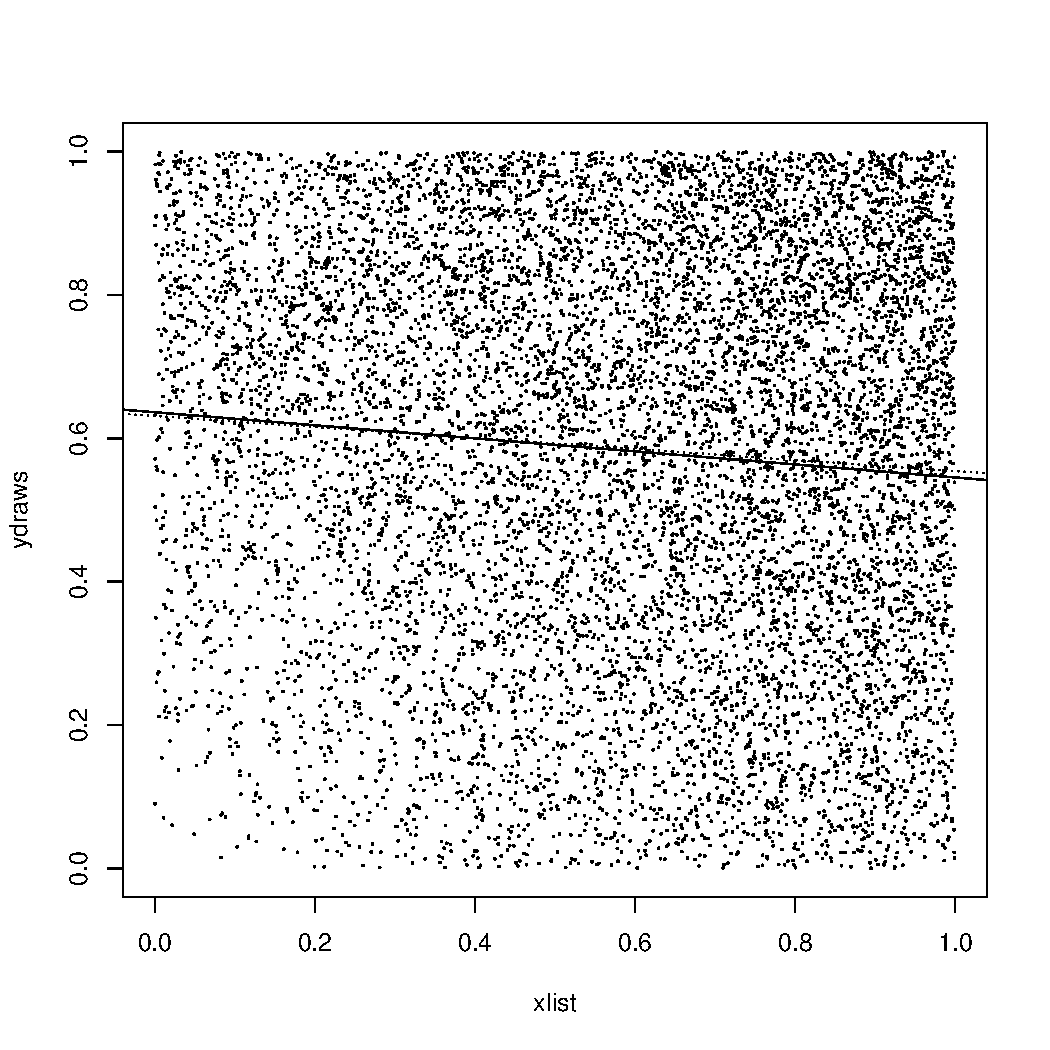
\includegraphics[width=4 in]{ConditionalExp.pdf}

\end{frame}

\begin{frame}
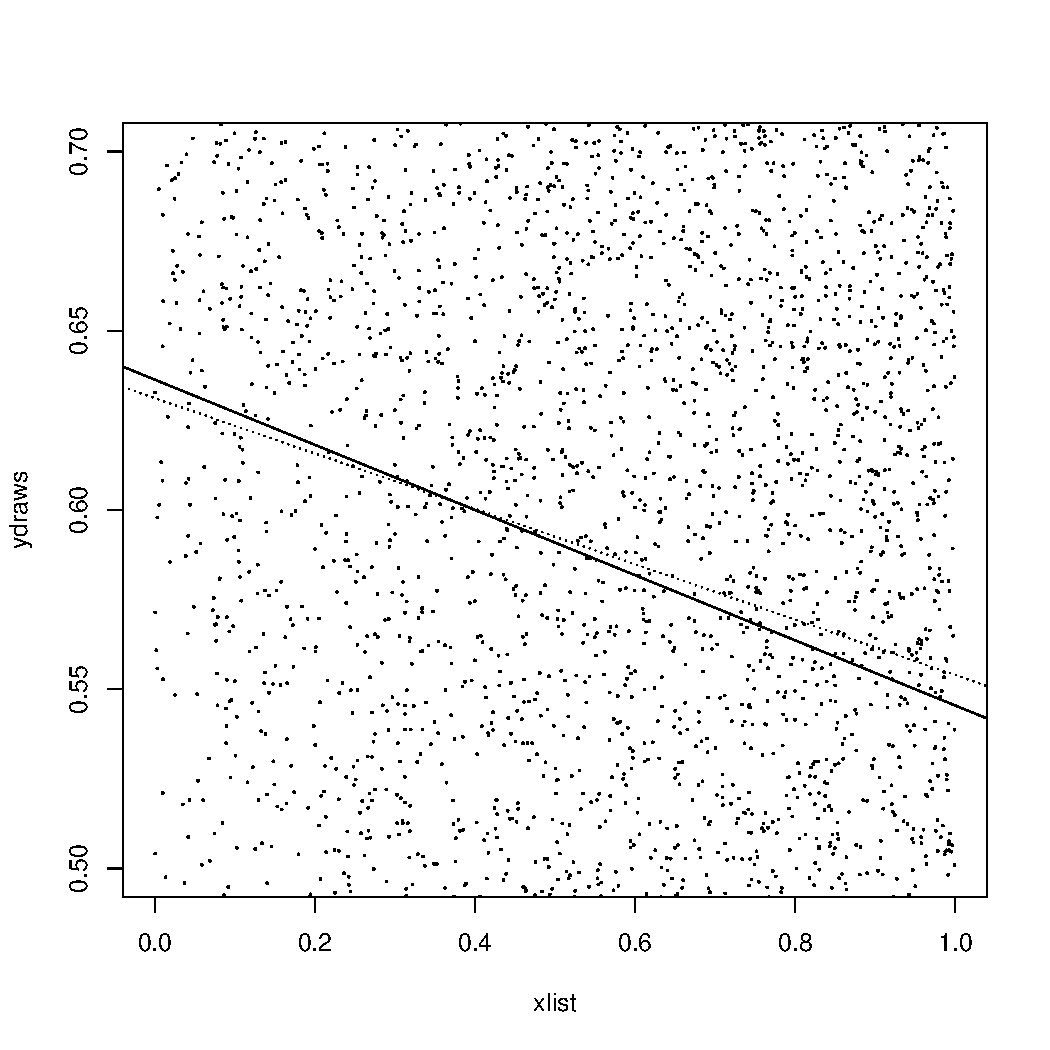
\includegraphics[width=4 in]{ConditionalExpZoom.pdf}

\end{frame}



\begin{frame}
\frametitle{Sums of Random Variables}

Suppose we have a sequence of random variables $X_{i}$ , $i = 1, 2, \hdots, N$.  \\

Suppose that they have joint pdf, 
\begin{eqnarray}
f(\boldsymbol{x}) & = & f(x_{1}, x_{2}, \hdots, x_{n}) \nonumber 
\end{eqnarray}

\begin{itemize}
\item[1)] $E[\sum_{i=1}^{N}X_{i} ]  = \sum_{i=1}^{N} E[X_{i}] $
\item[2)] var$(\sum_{i=1}^{N} X_{i} )   = \sum_{i=1}^{N} \text{var}(X_{i} )  + 2 \sum_{i<j} \text{cov}(X_{i}, X_{j}) $ 
\end{itemize}



\end{frame}


\begin{frame}
\frametitle{Sums of Random Variables}

\begin{prop}
Suppose we have a sequence of random variables $X_{i}$ , $i = 1, 2, \hdots, N$.  \\

Suppose that they have joint pdf, 
\begin{eqnarray}
f(\boldsymbol{x}) & = & f(x_{1}, x_{2}, \hdots, x_{n}) \nonumber 
\end{eqnarray}

Then 
\begin{eqnarray}
E[\sum_{i=1}^{N} X_{i} ] & = & \sum_{i=1}^{N} E[X_{i} ] \nonumber 
\end{eqnarray}

\end{prop}

\end{frame}


\begin{frame}

\begin{proof}

\begin{small}

\pause 
\begin{eqnarray}
\invisible<1>{E[\sum_{i=1}^{N} X_{i} ] & = &  E[X_{1} + X_{2} + \hdots + X_{N}] \nonumber \\} \pause 
\invisible<1-2>{& = & \int_{-\infty}^{\infty} \cdot \cdot \cdot \iint_{-\infty}^{\infty} (x_{1} + x_{2} + \hdots + x_{N}) f(x_{1}, x_{2}, \hdots, x_{N}) dx_{1}dx_{2}\hdots dx_{N} \nonumber \\} \pause 
\invisible<1-3>{& = & \int_{-\infty}^{\infty}x_{1} f_{X_{1}}(x_{1}) dx_{1}  + \int_{-\infty}^{\infty}x_{2} f_{X_{2}}(x_{2}) dx_{2} + \hdots + \int_{-\infty}^{\infty}x_{N} f_{X_{N}}(x_{N}) dx_{N}  \nonumber \\} \pause 
 \invisible<1-4>{& = & E[X_{1} ] + E[X_{2}] + \hdots + E[X_{N}] \nonumber } 
\end{eqnarray}

\end{small}

\end{proof}

\end{frame}


\begin{frame}
\frametitle{Sums of Random Variable}

\begin{prop}
Suppose $X_{i}$ is a sequence of random variables.  Then 

\begin{eqnarray}
\text{var}(\sum_{i=1}^{N} X_{i} ) & = & \sum_{i=1}^{N} \text{var}(X_{i} )  + 2 \sum_{i<j} \text{cov}(X_{i}, X_{j} ) \nonumber 
\end{eqnarray}

\end{prop}




\end{frame}


\begin{frame}
\frametitle{Sums of Random Variable}

\begin{proof}
Consider two random variables, $X_{1}$ and $X_{2}$.  Then, 

\pause 
\begin{eqnarray}
\invisible<1>{\text{var}(X_{1} + X_{2} ) & = & E[(X_{1} + X_{2})^2] - \left(E[X_{1}] + E[X_{2}] \right)^2 \nonumber \\ } \pause 
\invisible<1-2>{& = & E[X_{1}^2]  + 2 E[X_{1}X_{2}]  + E[X_{2}^2]  \nonumber \\
&& - (E[X_{1}])^2 - 2 E[X_{1}] E[X_{2}]  -  E[X_{2}]^2 \nonumber \\} \pause 
\invisible<1-3>{& = & \underbrace{E[X_{1}^2] - (E[X_{1}])^2}_{\text{var}(X_{1}) }   + \underbrace{E[X_{2}^2] - E[X_{2}]^{2}}_{\text{var}(X_{2})} \nonumber \\ 
&&  + 2 \underbrace{(E[X_{1} X_{2} ]  - E[X_{1}] E[X_{2} ] )}_{\text{cov}(X_{1}, X_{2} ) }  \nonumber \\} \pause 
 \invisible<1-4>{& = & \text{var}(X_{1} ) + \text{var}(X_{2} ) + 2 \text{cov}(X_{1}, X_{2}) \nonumber } 
\end{eqnarray}

\end{proof}

\end{frame}


\begin{frame}

\begin{defn}
Suppose $\boldsymbol{X} = (X_{1}, X_{2}, \hdots, X_{N}) $ is a vector of random variables.  If $\boldsymbol{X}$ has pdf 

\begin{eqnarray}
f(\boldsymbol{x}) & = & (2 \pi)^{-N/2} \text{det}\left(\boldsymbol{\Sigma}\right)^{-1/2} \exp\left(-\frac{1}{2}(\boldsymbol{x} - \boldsymbol{\mu})^{'}\boldsymbol{\Sigma} (\boldsymbol{x} - \boldsymbol{\mu} ) \right) \nonumber 
\end{eqnarray}
Then we will say $\boldsymbol{X}$ is a \alert{Multivariate Normal} Distribution, 
\begin{eqnarray}
\boldsymbol{X} & \sim & \text{Multivariate Normal} (\boldsymbol{\mu}, \boldsymbol{\Sigma}) \nonumber 
\end{eqnarray}


\end{defn}

\begin{itemize}
\item[-] \alert{Regularly} used for likelihood, Bayesian, and other parametric inferences
\end{itemize}



\end{frame}


\begin{frame}
\frametitle{Multivariate Normal Distribution}

Consider the (bivariate) special case where $\boldsymbol{\mu} = (0, 0)$ and 
\begin{eqnarray}
\boldsymbol{\Sigma} & = & \begin{pmatrix} 
1 & 0 \\
0 & 1 \\
\end{pmatrix}
\nonumber 
\end{eqnarray}

\pause 
\invisible<1>{Then 
\begin{eqnarray}
f(x_{1}, x_{2} ) & = & (2\pi)^{-2/2} 1^{-1/2} \exp\left(-\frac{1}{2}\left( (\boldsymbol{x}  - \boldsymbol{0} ) ^{'} \begin{pmatrix} 
1 & 0 \\
0 & 1 \\
\end{pmatrix}
(\boldsymbol{x}  - \boldsymbol{0} ) \right) \right) \nonumber \\} \pause 
 \invisible<1-2>{& = & \frac{1}{2\pi} \exp\left(-\frac{1}{2} (x_{1}^{2} + x_{2} ^ 2 )     \right) \nonumber \\} \pause 
 \invisible<1-3>{& = & \frac{1}{\sqrt{2\pi}} \exp\left(-\frac{x_{1}^{2}}{2}  \right) \frac{1}{\sqrt{2\pi}} \exp\left(-\frac{x_{2}^{2}}{2}  \right) \nonumber} \pause 
\end{eqnarray}

\invisible<1-4>{$\leadsto$ product of univariate standard normally distributed random variables} 

\end{frame}


\begin{frame}
\frametitle{Standard Multivariate Normal}

\begin{defn}

Suppose $\boldsymbol{Z} = (Z_{1}, Z_{2}, \hdots, Z_{N}) $ is 
\begin{eqnarray}
\boldsymbol{Z} & \sim & \text{Multivariate Normal}(\boldsymbol{0}, \boldsymbol{I}_{N} ) . \nonumber
\end{eqnarray}

Then we will call $\boldsymbol{Z}$ the standard multivariate normal.  
\end{defn}



\end{frame}

\begin{frame}
\frametitle{Properties of the Multivariate Normal Distribution}

Suppose $\boldsymbol{X} = (X_{1}, X_{2}, \hdots, X_{N} ) $

\begin{eqnarray}
E[\boldsymbol{X} ] & = &  \boldsymbol{\mu}\nonumber \\
\text{cov}(\boldsymbol{X} ) & = & \boldsymbol{\Sigma} \nonumber 
\end{eqnarray}

So that, 

\begin{eqnarray}
\boldsymbol{\Sigma}  & = & \begin{pmatrix} 
\text{var}(X_{1}) & \text{cov}(X_{1}, X_{2}) & \hdots & \text{cov}(X_{1}, X_{N}) \\
\text{cov}(X_{2}, X_{1}) & \text{var}(X_{2}) & \hdots & \text{cov}(X_{2}, X_{N} ) \\
\vdots & \vdots & \ddots & \vdots \\
\text{cov}(X_{N}, X_{1} ) & \text{cov}(X_{N}, X_{2} ) & \hdots & \text{var}(X_{N} ) \\
\end{pmatrix} \nonumber 
\end{eqnarray}


\end{frame}


\begin{frame}
\frametitle{Independence and Multivariate Normal}

\begin{prop}
Suppose $X$ and $Y$ are independent.  Then 
\begin{eqnarray}
\text{cov}(X, Y) & = & 0 \nonumber 
\end{eqnarray}

\end{prop}



\end{frame}


\begin{frame}
\begin{small}
\begin{proof}
Suppose $X$ and $Y$ are independent.  \pause 
\begin{eqnarray}
\invisible<1>{\text{cov}(X, Y) & = & E[XY] - E[X]E[Y] \nonumber } \pause 
\end{eqnarray}

\invisible<1-2>{Calculating $E[XY]$} \pause 
\begin{eqnarray}
\invisible<1-3>{E[XY] & = & \int_{-\infty}^{\infty} \int_{-\infty}^{\infty} x y f(x,y)dxdy \nonumber \\} \pause 
\invisible<1-4>{& =& \int_{-\infty}^{\infty} \int_{-\infty}^{\infty} x y f_{X}(x) f_{Y}(y)dxdy \nonumber \\} \pause 
\invisible<1-5>{& = & \int_{-\infty}^{\infty} x f_{X}(x) dx \int_{-\infty}^{\infty} y f_{Y}(y) dy \nonumber \\} \pause 
 \invisible<1-6>{& = & E[X] E[Y] \nonumber} \pause 
\end{eqnarray}

\invisible<1-7>{Then cov$(X,Y) = 0$.} 


\end{proof}

\end{small}


\end{frame}


\begin{frame}
\frametitle{Zero covariance does not \alert{generally} imply Independent}
Suppose $X \in \{-1, 1\}$ with $P(X = 1) = P(X = -1) = 1/2$.  \\
Suppose $Y \in \{-1, 0,1\}$ with $Y = 0 $ if $X = -1$ and $P(Y = 1) = P(Y= -1) $ if $X = 1$.  \\

\begin{small}
\begin{eqnarray}
E[XY] & = & \sum_{i \in \{-1, 1\} } \sum_{j \in \{-1, 0, 1\}} i j P(X = i, Y = j) \nonumber \\
& = & -1 \times 0 \times  P(X = -1, Y = 0) + 1 \times 1  \times P(X = 1, Y = 1)  \nonumber \\
 && - 1 \times 1 \times P(X = 1, Y = -1) \nonumber \\
 &= & 0 + P(X = 1, Y = 1)  - P(X = 1, Y = -1 ) \nonumber \\
  & = &  0.25 - 0.25 = 0  \nonumber \\
E[X] & = &  0 \nonumber \\
E[Y] & = & 0 \nonumber 
\end{eqnarray}

\end{small}



\end{frame}


\begin{frame}

\begin{prop}
Suppose $\boldsymbol{X} \sim \text{Multivariate Normal}(\boldsymbol{\mu}, \boldsymbol{\Sigma})$.  
where $\boldsymbol{X}= (X_{1}, X_{2}, \hdots, X_{N})$. \\
If $\text{cov}(X_{i}, X_{j})  = 0  $, then $X_{i}$ and $X_{j}$ are independent 

\end{prop}



\end{frame}



\begin{frame}
\frametitle{Iterated Expectations}

\begin{prop}
Suppose $X$ and $Y$ are random variables.  Then 

\begin{eqnarray}
E[X] & = & E[E[X|Y]] \nonumber 
\end{eqnarray}




\end{prop}


\begin{itemize}
\item[-] Inner Expectation is $E[X|Y] = \int_{-\infty}^{\infty} x f_{X|Y} (x|y) dx$.  
\item[-] Outer expectation is over $y$.  
\end{itemize}


\end{frame}


\begin{frame}
\frametitle{Iterated Expectations}

\pause 
\begin{proof}
\begin{eqnarray}
\invisible<1>{E[E[X|Y]] & = & \int_{-\infty}^{\infty}  \int_{-\infty}^{\infty} x f_{X|Y} (x|y) f_{Y}(y) dx dy \nonumber \\} \pause 
 \invisible<1-2>{&= & \int_{-\infty}^{\infty}  \int_{-\infty}^{\infty} x f_{X|Y} (x|y) f_{Y}(y) dy dx \nonumber \\} \pause 
 \invisible<1-3>{& = & \int_{-\infty}^{\infty} x \int_{-\infty}^{\infty}  f(x, y) dy dx  \nonumber \\} \pause 
 \invisible<1-4>{& = & \int_{-\infty}^{\infty}  x f_{X}(x) dx  \nonumber \\} \pause 
  \invisible<1-5>{& =& E[X] \nonumber } 
\end{eqnarray}



\end{proof}



\end{frame}


\begin{frame}
\frametitle{Iterated Expectations}

\begin{defn}
Suppose $Y$ is a continuous random variable with $Y \in [0,1]$ and pdf of $Y$ given by 

\begin{eqnarray}
f(y) & = & \frac{\Gamma(\alpha_1 + \alpha_2)}{\Gamma(\alpha_{1} ) \Gamma(\alpha_{2})} y^{\alpha_{1} - 1} (1- y)^{\alpha_{2} - 1 } \nonumber 
\end{eqnarray}

Then we will say $Y$ is a \alert{Beta} distribution with parameters $\alpha_{1}$ and $\alpha_{2}$.  Equivalently,
\begin{eqnarray}
Y & \sim & \text{Beta}(\alpha_{1}, \alpha_{2} ) \nonumber 
\end{eqnarray}



\end{defn}


\begin{itemize}
\item[-] Beta is a distribution on \alert{proportions} 
\item[-] Beta is a special case of the \alert{Dirichlet} distribution 
\item[-] $E[Y] = \frac{\alpha_{1}}{\alpha_{1} + \alpha_{2}}$
\end{itemize}


\end{frame}


\begin{frame}
\frametitle{Iterated Expectations}

Suppose 
\begin{eqnarray}
\pi & \sim & \text{Beta}(\alpha_{1}, \alpha_{2}) \nonumber \\
Y|\pi, n & \sim & \text{Binomial}(n, \pi)\nonumber 
\end{eqnarray}

What is $E[Y]$? \pause 

\begin{eqnarray}
\invisible<1>{E[Y] & = & E[E[Y| \pi]] \nonumber \\} \pause 
\invisible<1-2>{& = & \int_{-\infty}^{\infty} \sum_{j = 0}^{N} {{N}\choose{j}} j p(j|\pi) f(\pi) d\pi \nonumber \\} \pause 
\invisible<1-3>{ & = & \int_{-\infty}^{\infty} N \pi f(\pi) d\pi \nonumber  \\} \pause 
  \invisible<1-4>{& = & N \frac{\alpha_{1}}{\alpha_{1} + \alpha_{2}} \nonumber } 
\end{eqnarray}


\end{frame}


\begin{frame}
\frametitle{Conditional Expectation as an Estimator}
Suppose $Y$ is a random variable, and $X$ is some data.

\begin{eqnarray}
\hat{Y} & = & E[Y|X] \nonumber 
\end{eqnarray}\pause
So we know $\hat{Y}$ is an estimator.\\


\end{frame}


\begin{frame}
\frametitle{Estimation error}
Suppose $\hat{Y}$ is an estimator from before, the estimation error:
\begin{eqnarray}
\tilde{Y} & = & \hat{Y}-Y \nonumber 
\end{eqnarray}\pause
is a random variable where:
\begin{eqnarray}
E[\tilde{Y}|X] & = & E[ \hat{Y}-Y|X]=E[ \hat{Y}|X]-E[Y|X]=\hat{Y} -\hat{Y} =0\nonumber 
\end{eqnarray}\pause
By iterated expectations:\pause
\begin{eqnarray}
E[\tilde{Y}] & = & E[E[ \tilde{Y}|X]]=0 \nonumber 
\end{eqnarray}\pause
This estimators error centers on 0.

\end{frame}


\begin{frame}
\frametitle{Correlation of  Estimator and Estimation Error}
Suppose $\hat{Y}$ is an estimator from before, and $\tilde{Y}$ the estimation error.
\begin{eqnarray}
E[\tilde{Y}\hat{Y}] & = & E[E[\tilde{Y}\hat{Y}|X]]=E[\hat{Y}E[\tilde{Y}|X]]=0 \nonumber 
\end{eqnarray}\pause
because $\hat{Y}$ only depends on $X$.\pause
\begin{eqnarray}
cov(\tilde{Y},\hat{Y}) & = & E[ \tilde{Y}\hat{Y}]-E[\tilde{Y}]E[\hat{Y}]=0- E[\tilde{Y}]0=0\nonumber 
\end{eqnarray}\pause
The error is uncorrelated with the estimate.  This is what allows us to separate the signal from the noise.
\end{frame}


\begin{frame}
\frametitle{Law of Total Variance}
Suppose $X$ and $Y$ are random variables.  Then 

\begin{eqnarray}
var[X] & = & E[var[X|Y]]+var(E[X|Y]) \nonumber 
\end{eqnarray}
The first term is the average of the variation for each value of Y.\pause
The second term is the variation across the averages within each value of Y.
\end{frame}

\begin{frame}
\frametitle{Law of Total Variance: application}
Suppose $\theta$ is a parameter, and $x$ is data.

\begin{eqnarray}
var[\theta] & = & E[var[\theta|x]]+var(E[\theta|x]) \nonumber 
\end{eqnarray}
The expected variance of $\theta$ conditional on data (the posterior) is less than the variance in $\theta$ without the data (the prior).
\end{frame}


\end{document}